\section{\trMarkedSimplicialSet{}与\trMarkedAnodyne{}映射}
\label{sec:marked-simplicial-sets}

迄今为止，我们已经看到，\trLeftFibration{}/\trRightFibration{}是一种特殊类型的%
（余）\trCartesianFibration{}。既然\trLeftFibration{}由一个\trRightLiftingProperty{}%
（相对于\trLeftAnodyne{}映射）确定，人们自然会问：（余）\trCartesianFibration{}是否也由某个%
提升性质刻画。答案是：这并不严格成立，但在\trMarkedSimplicialSet{}的语境中成立；
所谓\trMarkedSimplicialSet{}，是指把一族 $1$-\trSimplex{}（带标记的边）作为数据的
一部分牢记在心的\trSimplicialSet{}。

\trMarkedSimplicialSet{}为∞-\trCategories{}的∞-\trCategory{}提供了另一个模型。
尽管这一表现方式比若亚尔\trModelStructure{}具有某些技术上的优势，但这一点对我们
来说并不十分重要。然而，我们将把\trMarkedSimplicialSet{}与前文的\trDwyer{}--%
\trKan{}\trLocalization{}构造联系起来，也就是说，\trDwyer{}--\trKan{}%
\trLocalization{}与\trMarkedEquivalence{}之间存在着紧密的联系，并且我们将看到，指向一个%
\trDwyer{}--\trKan{}\trLocalization{}的典范映射可以被看作\trMarkedSimplicialSet{}上%
的带标记\trModelStructure{}中的纤维性替换。

\begin{definition}\label{def:marked-simplicial-set}
一个\emph{\trMarkedSimplicialSet{}}（marked simplicial set）是一个二元组
$(X, M)$，其中 $M$ 是 $X$ 的诸 $1$-\trSimplex{} 的一个子集，它包含所有退化的
$1$-\trSimplex{}。$M$ 的元素称为 $X$ 中的\emph{\trMarkedEdge{}}（marked edge）。注意，
存在一个相应的带标记\trSimplicialSet{}的\trCategory{} $\mathrm{sSet}_+$，其中的%
\trMorphism{}被要求把\trMarkedEdge{}送到\trMarkedEdge{}。
\end{definition}

\begin{example*}
设 $X$ 是一个\trSimplicialSet{}。我们用 $X^\flat$ 表示这样一个%
\trMarkedSimplicialSet{}，其中一条边带标记，当且仅当它是退化的；用 $X^\sharp$
表示其中所有\trMorphism{}都带标记的那个\trMarkedSimplicialSet{}。这就产生了%
\trFunctor{} $(-)^\flat$ 与 $(-)^\sharp\colon \mathrm{sSet} \to \mathrm{sSet}_+$。
还有两个\trFunctor{} $\mathrm{sSet}_+ \to \mathrm{sSet}$：其中一个遗忘标记，
另一个取由带标记的 $1$-\trSimplex{} 张成的最小子\trSimplicialSet{}。
\end{example*}

\begin{example*}
设 $p\colon X \to S$ 是\trSimplicialSet{}之间的一个映射。我们用 $X^\natural$
表示这样一个\trMarkedSimplicialSet{}，其中一条边带标记，当且仅当它是
$p$-余笛卡尔的。于是，如果 $p\colon X \to S$ 是一个\trCocartesianFibration{}，
那么映射 $X^\natural \to S^\sharp$ 就是带标记\trSimplicialSet{}之间的一个映射。
\end{example*}

\begin{definition}\label{def:marked-left-anodyne}
包含下列带标记\trSimplicialSet{}之间的映射的最小\trSaturatedSet{}称为%
\emph{\trMarkedLeftAnodyne}（marked left-anodyne）：
\begin{enumerate}[label=(\arabic*)]
  \item 对一切 $0 < i < n$，映射 $(\Lambda^n_i)^\flat \to (\Delta^n)^\flat$；
  \item 对每个 $n > 0$，映射 $(\Lambda^n_0)^{s\flat} \to (\Delta^n)^{s\flat}$，
        其中上标 $s\flat$ 表示所有退化的边与特殊的边 $\Delta^{\{0,1\}}$ 均带标记；
  \item 映射 $(\Lambda^2_1)^\sharp \amalg_{(\Lambda^2_1)^\flat} (\Delta^2)^\flat \to (\Delta^2)^\sharp$；以及
  \item 对每个∞-\trGroupoid{} $X$，映射 $X^\flat \to X^\sharp$。
\end{enumerate}
\end{definition}

\begin{remark}\label{rem:marked-left-anodyne-generators}
\trMarkedLeftAnodyne{}映射的一个不同的（但等价的）生成集由以下映射给出：
\begin{enumerate}[label={(\arabic*)$'$}]
  \item 对一切 $0 < i < n$，映射 $(\Lambda^n_i)^\flat \to (\Delta^n)^\flat$；
  \item 映射 $(\Delta^1)^\sharp \times (\Delta^1)^\flat \cup \{0\} \times (\Delta^1)^\sharp \to (\Delta^1)^\sharp \times (\Delta^1)^\sharp$；
  \item 映射 $(\Delta^1)^\sharp \times (\partial\Delta^n)^\flat \cup \{0\} \times (\Delta^n)^\flat \to (\Delta^1)^\sharp \times (\Delta^n)^\flat$；
  \item 映射 $J^\flat \to J^\sharp$。
\end{enumerate}
\end{remark}

\begin{remark}\label{rem:marked-left-anodyne-equivalent-generators}
我们同样可以取由映射 (1)、(2)、(3$'$) 与 (4) 生成的那个集合，细节见
\cite[Proposition 3.1.1.5]{Lur09}。这将在\cref{lem:pushout-product-marked-left-anodyne}中
用到。类似地，我们也可以使用由 (1)、(2)、(3) 与 (4$'$) 生成的集合。（事实上，
这一点非常容易看出，我们推荐把它当作一道练习。）
\end{remark}

为了证明（余）\trCartesianFibration{}在\trMarkedSimplicialSet{}的语境中由一个提升性质确定，
方便的做法是先谈论\trLocallyCocartesian{}边。

\begin{definition}\label{def:locally-cocartesian}
设 $p\colon X \to S$ 是\trSimplicialSet{}之间的一个\trInnerFibration{}。一条边
$f\colon x \to y$ 称为\emph{\trLocallyCocartesian}（locally cocartesian），如果它是
$q$-余笛卡尔的，其中 $q$ 是如下\trPullback{}%
\begin{center}
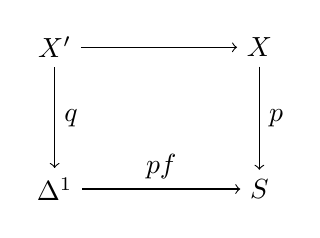
\begin{tikzpicture}
  \node (xp) at (0,0) {$X'$};
  \node (x) at (2.6,0) {$X$};
  \node (d1) at (0,-1.8) {$\Delta^1$};
  \node (s) at (2.6,-1.8) {$S$};
  \draw[->] (xp) -- (x);
  \draw[->] (xp) -- node[right] {$q$} (d1);
  \draw[->] (x) -- node[right] {$p$} (s);
  \draw[->] (d1) -- node[above] {$pf$} (s);
\end{tikzpicture}
\end{center}
\end{definition}

\begin{lemma}\label{lem:locally-cocartesian}
设 $p\colon X \to S$ 是一个\trInnerFibration{}，并设 $f\colon x \to y$ 是 $X$
中的一条边。
\begin{enumerate}[label=(\arabic*)]
  \item 如果 $f$ 是 $p$-余笛卡尔的，那么它是\trLocallyCocartesian。
  \item 如果 $f$ 是\trLocallyCocartesian，并且存在 $p(f)$ 的一个 $p$-余笛卡尔提升
        $g\colon x \to y'$，那么 $f$ 是 $p$-余笛卡尔的。
\end{enumerate}
\end{lemma}

\begin{proof}
事实上，陈述 (1) 可以加强为：如果 $f$ 相对于 $p$ 的某个\trPullback{}是
$p'$-余笛卡尔的，那么 $f$ 就是\trLocallyCocartesian，见\cref{ex:p-prime-cocartesian-locally-cocartesian}。我们在此省去其证明。
为了证明 (2)，我们考虑\trLiftingProblem{}%
\begin{center}
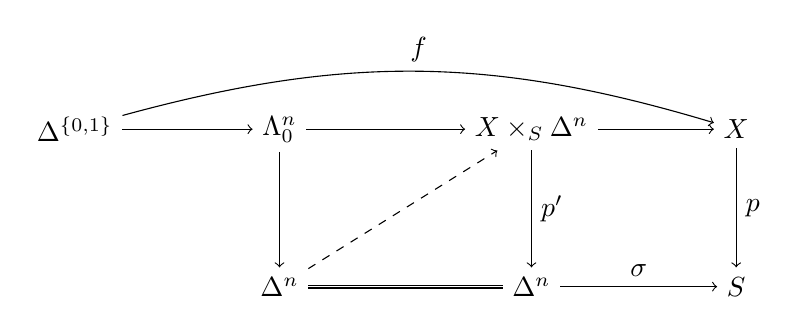
\begin{tikzpicture}
  \node (d01) at (0,0) {$\Delta^{\{0,1\}}$};
  \node (horn) at (2.6,0) {$\Lambda^n_0$};
  \node (pb) at (5.8,0) {$X \times_S \Delta^n$};
  \node (x) at (8.4,0) {$X$};
  \node (dn1) at (2.6,-2) {$\Delta^n$};
  \node (dn2) at (5.8,-2) {$\Delta^n$};
  \node (s) at (8.4,-2) {$S$};
  \draw[->] (d01) -- (horn);
  \draw[->] (horn) -- (pb);
  \draw[->] (pb) -- (x);
  \draw[->] (horn) -- (dn1);
  \draw[->] (pb) -- node[right] {$p'$} (dn2);
  \draw[->] (x) -- node[right] {$p$} (s);
  \draw[double] (dn1) -- (dn2);
  \draw[->] (dn2) -- node[above] {$\sigma$} (s);
  \draw[->, dashed] (dn1) -- (pb);
  \draw[->, bend left=16] (d01) to node[above] {$f$} (x);
\end{tikzpicture}
\end{center}
记 $X' = X \times_S \Delta^n$。我们观察到，$f$ 与 $g$ 都典范地是 $X'$ 中的边，
其中 $f$ 仍是\trLocallyCocartesian，而 $g$ 是 $p'$-余笛卡尔的。为了看出 $g$ 的确给出
$X'$ 的一条边，我们只需观察图表
\begin{center}
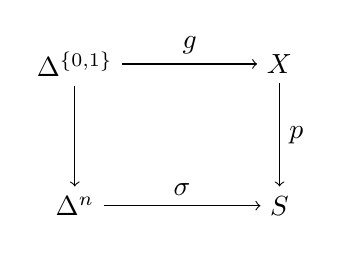
\begin{tikzpicture}
  \node (d01) at (0,0) {$\Delta^{\{0,1\}}$};
  \node (x) at (2.6,0) {$X$};
  \node (dn) at (0,-1.8) {$\Delta^n$};
  \node (s) at (2.6,-1.8) {$S$};
  \draw[->] (d01) -- node[above] {$g$} (x);
  \draw[->] (d01) -- (dn);
  \draw[->] (x) -- node[right] {$p$} (s);
  \draw[->] (dn) -- node[above] {$\sigma$} (s);
\end{tikzpicture}
\end{center}
交换。于是我们可以假设 $S$ 是一个∞-\trCategory{}。在这种情形下，我们考虑由 $g$
与 $f$ 得到的角，以及\trLiftingProblem{}%
\begin{center}
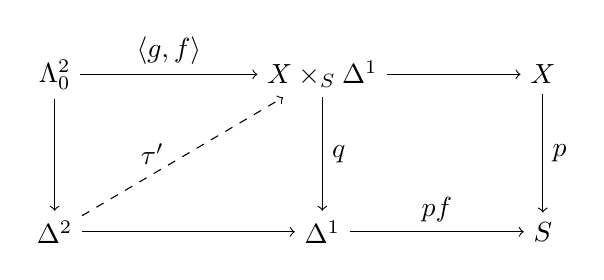
\begin{tikzpicture}
  \node (horn) at (0,0) {$\Lambda^2_0$};
  \node (pb) at (3.4,0) {$X \times_S \Delta^1$};
  \node (x) at (6.2,0) {$X$};
  \node (d2) at (0,-2) {$\Delta^2$};
  \node (d1) at (3.4,-2) {$\Delta^1$};
  \node (s) at (6.2,-2) {$S$};
  \draw[->] (horn) -- node[above] {$\langle g, f\rangle$} (pb);
  \draw[->] (pb) -- (x);
  \draw[->] (horn) -- (d2);
  \draw[->] (pb) -- node[right] {$q$} (d1);
  \draw[->] (x) -- node[right] {$p$} (s);
  \draw[->] (d2) -- (d1);
  \draw[->] (d1) -- node[above] {$pf$} (s);
  \draw[->, dashed] (d2) -- node[above, pos=0.35] {$\tau'$} (pb);
\end{tikzpicture}
\end{center}
由于 $g$ 是 $p$-余笛卡尔的，一个使图表交换的虚线箭头存在。我们断言，
$h = \tau'|_{\Delta^{\{1,2\}}}$ 是纤维∞-\trCategory{} $X_{p(y)}$ 中的一个%
\trEquivalence{}。由\cref{lem:cartesian-three-for-two}，我们可以推出 $h$ 是
$q$-余笛卡尔的且位于恒等之上。于是，由\cref{lem:equivalence-cartesian}，它是纤维
$X_{p(y)}$ 中的一个\trEquivalence{}。再由\cref{lem:equivalence-cartesian}，我们
推出 $h$ 也是 $p$-余笛卡尔的。（注意，我们已经假设了 $S$ 从而 $X$ 是
∞-\trCategories{}。）
\end{proof}

下述引理给出另一个有用的观察。

\begin{lemma}\label{lem:locally-cocartesian-two-out-of-three}
设 $p\colon X \to S$ 是\trSimplicialSet{}之间的一个\trInnerFibration{}。考虑 $X$
的一个描绘成如下图表的 $2$-\trSimplex{}%
\begin{center}
\begin{tikzpicture}
  \node (y) at (2.2,0) {$y$};
  \node (x) at (0,-1.8) {$x$};
  \node (z) at (4.4,-1.8) {$z$};
  \draw[->] (x) -- node[above, pos=0.35] {$f$} (y);
  \draw[->] (y) -- node[above right, pos=0.4] {$g$} (z);
  \draw[->] (x) -- node[below] {$h$} (z);
\end{tikzpicture}
\end{center}
假设 $f$ 是 $p$-余笛卡尔的。那么，如果 $g$（相应地，$h$）是 $p$-余笛卡尔的，
则 $h$（相应地，$g$）是\trLocallyCocartesian。
\end{lemma}

\begin{proof}
\cref{ex:prove-lemma-3-2-7}。
\end{proof}

\begin{remark}\label{rem:rezk-locally-cocartesian}
在 \cite{Rez19} 中，你可以找到关于局部（余）笛卡尔边的更多信息，以及判定局部%
（余）笛卡尔边何时事实上是（余）笛卡尔的若干准则。
\end{remark}

\begin{proposition}\label{prop:marked-rlp-characterization}
带标记\trSimplicialSet{}之间的一个映射 $p\colon X \to S$ 相对于所有%
\trMarkedLeftAnodyne{}映射具有\trRightLiftingProperty{}，当且仅当下列各点成立：
\begin{enumerate}[label=(\arabic*)]
  \item $p$ 是一个\trInnerFibration{}。
  \item $X$ 的一条边带标记，当且仅当它是 $p$-余笛卡尔的，且它在 $S$ 中的像带标记。
  \item \trMarkedSimplicialSet{}的任何\trLiftingProblem{}%
\begin{center}
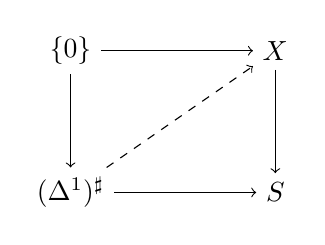
\begin{tikzpicture}
  \node (pt) at (0,0) {$\{0\}$};
  \node (x) at (2.6,0) {$X$};
  \node (d1) at (0,-1.8) {$(\Delta^1)^\sharp$};
  \node (s) at (2.6,-1.8) {$S$};
  \draw[->] (pt) -- (x);
  \draw[->] (pt) -- (d1);
  \draw[->] (d1) -- (s);
  \draw[->] (x) -- (s);
  \draw[->, dashed] (d1) -- (x);
\end{tikzpicture}
\end{center}
        可解。
\end{enumerate}
\end{proposition}

\begin{proof}
让我们首先假设 $p$ 相对于\trMarkedLeftAnodyne{}映射满足 RLP，并推出 $p$ 满足陈述中的条件
(1) 至 (3)。性质 (1) 与 (3) 容易得出。为了看出 (2)，我们首先证明任何\trMarkedEdge{}%
$f\colon (\Delta^1)^\sharp \to X$ 都是 $p$-余笛卡尔的。为此，考虑\trLiftingProblem{}%
\begin{center}
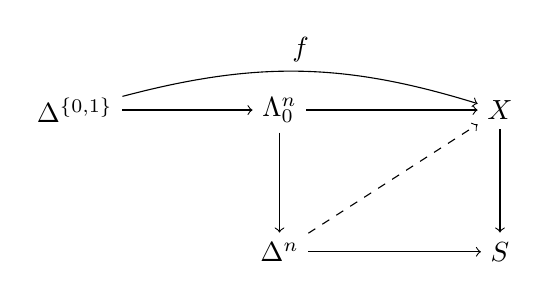
\begin{tikzpicture}
  \node (d01) at (0,0) {$\Delta^{\{0,1\}}$};
  \node (horn) at (2.6,0) {$\Lambda^n_0$};
  \node (x) at (5.4,0) {$X$};
  \node (dn) at (2.6,-1.8) {$\Delta^n$};
  \node (s) at (5.4,-1.8) {$S$};
  \draw[->] (d01) -- (horn);
  \draw[->] (horn) -- (x);
  \draw[->] (horn) -- (dn);
  \draw[->] (dn) -- (s);
  \draw[->] (x) -- (s);
  \draw[->, dashed] (dn) -- (x);
  \draw[->, bend left=16] (d01) to node[above] {$f$} (x);
\end{tikzpicture}
\end{center}
我们想证明这个\trLiftingProblem{}容有一个解：由于上述复合是带标记的，它给出一个%
带标记\trSimplicialSet{}的图表
\begin{center}
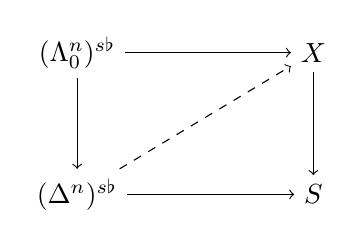
\begin{tikzpicture}
  \node (horn) at (0,0) {$(\Lambda^n_0)^{s\flat}$};
  \node (x) at (3,0) {$X$};
  \node (dn) at (0,-1.8) {$(\Delta^n)^{s\flat}$};
  \node (s) at (3,-1.8) {$S$};
  \draw[->] (horn) -- (x);
  \draw[->] (horn) -- (dn);
  \draw[->] (dn) -- (s);
  \draw[->] (x) -- (s);
  \draw[->, dashed] (dn) -- (x);
\end{tikzpicture}
\end{center}
它可以求解，因为左边的竖直映射是\trMarkedAnodyne{}的。

反过来，接下来我们证明：只要 $pf$ 带标记，任何 $p$-余笛卡尔的边 $f\colon x \to y$
就都带标记。为此，考虑图表
\begin{center}
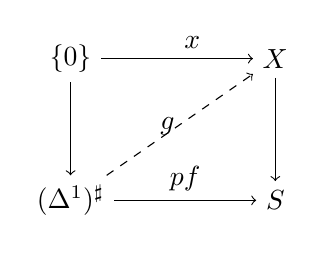
\begin{tikzpicture}
  \node (pt) at (0,0) {$\{0\}$};
  \node (x) at (2.6,0) {$X$};
  \node (d1) at (0,-1.8) {$(\Delta^1)^\sharp$};
  \node (s) at (2.6,-1.8) {$S$};
  \draw[->] (pt) -- node[above, pos=0.6] {$x$} (x);
  \draw[->] (pt) -- (d1);
  \draw[->] (d1) -- node[above] {$pf$} (s);
  \draw[->] (x) -- (s);
  \draw[->, dashed] (d1) -- node[above right, pos=0.3] {$g$} (x);
\end{tikzpicture}
\end{center}
由假设它可以求解。所得的\trMorphism{} $g$ 是带标记的，从而由前面的论证它是
$p$-余笛卡尔的。进而考虑图表
\begin{center}
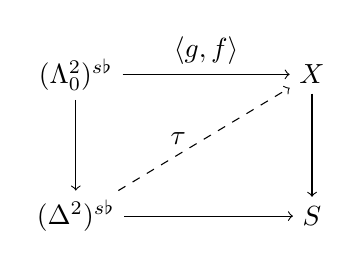
\begin{tikzpicture}
  \node (horn) at (0,0) {$(\Lambda^2_0)^{s\flat}$};
  \node (x) at (3,0) {$X$};
  \node (d2) at (0,-1.8) {$(\Delta^2)^{s\flat}$};
  \node (s) at (3,-1.8) {$S$};
  \draw[->] (horn) -- node[above] {$\langle g, f\rangle$} (x);
  \draw[->] (horn) -- (d2);
  \draw[->] (d2) -- (s);
  \draw[->] (x) -- (s);
  \draw[->, dashed] (d2) -- node[above, pos=0.35] {$\tau$} (x);
\end{tikzpicture}
\end{center}
由假设它同样可以求解。这里，下面的水平映射是\trMorphism{} $pf = pg$ 上的一个退化
$2$-\trSimplex{}。我们把 $\tau|_{\Delta^{\{1,2\}}}$ 记为 $h$。考虑\trPullback{}图表
\begin{center}
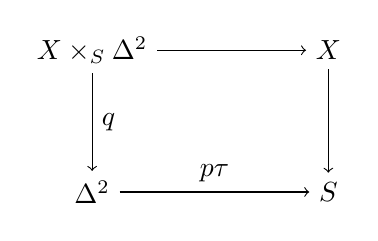
\begin{tikzpicture}
  \node (pb) at (0,0) {$X \times_S \Delta^2$};
  \node (x) at (3,0) {$X$};
  \node (d2) at (0,-1.8) {$\Delta^2$};
  \node (s) at (3,-1.8) {$S$};
  \draw[->] (pb) -- (x);
  \draw[->] (pb) -- node[right] {$q$} (d2);
  \draw[->] (x) -- (s);
  \draw[->] (d2) -- node[above] {$p\tau$} (s);
\end{tikzpicture}
\end{center}
以及典范映射 $\Delta^2 \to X \times_S \Delta^2$%
\footnote{译注：原书两处印作 $X \times_Y \Delta^2$，但本节中并未出现任何 $Y$；
按上述\trPullback{}图表，$q$ 是 $p$ 沿 $p\tau\colon \Delta^2 \to S$ 的拉回，故应为
$X \times_S \Delta^2$，兹径改。——译者注}，我们可以应用\cref{lem:cartesian-three-for-two}
看出 $h$ 是 $q$-余笛卡尔的，因为 $f$ 与 $g$ 也都是 $q$-余笛卡尔的。由于
$qh = \mathrm{id}_{p(y)}$，我们从\cref{lem:equivalence-cartesian}推出 $h$ 是
∞-\trCategory{} $X_{p(y)}$ 中的一个\trEquivalence{}。我们考虑图表
\begin{center}
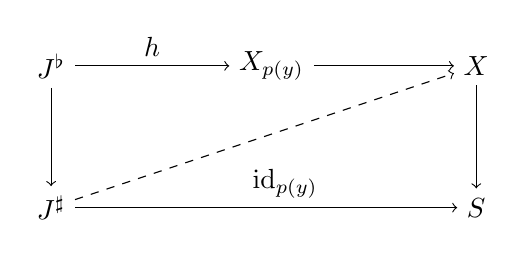
\begin{tikzpicture}
  \node (jb) at (0,0) {$J^\flat$};
  \node (fib) at (2.8,0) {$X_{p(y)}$};
  \node (x) at (5.4,0) {$X$};
  \node (js) at (0,-1.8) {$J^\sharp$};
  \node (s) at (5.4,-1.8) {$S$};
  \draw[->] (jb) -- node[above] {$h$} (fib);
  \draw[->] (fib) -- (x);
  \draw[->] (jb) -- (js);
  \draw[->] (js) -- node[above, pos=0.55] {$\mathrm{id}_{p(y)}$} (s);
  \draw[->] (x) -- (s);
  \draw[->, dashed] (js) -- (x);
\end{tikzpicture}
\end{center}
它也可以求解，因为 $J$ 是一个∞-\trGroupoid{}。由此得出 $h$ 是带标记的。接下来，
我们观察到，相对于映射 $(\Lambda^2_1)^\sharp \amalg_{(\Lambda^2_1)^\flat} (\Delta^2)^\flat \to (\Delta^2)^\sharp$ 的 RLP 蕴含：带标记\trMorphism{}的合成是带标记的。由于
$f$ 是 $g$ 与 $h$ 的一个合成，我们发现 $f$ 正如所需是带标记的。

我们现在证明：任何满足陈述中性质 (1) 至 (3) 的带标记\trSimplicialSet{}的映射
$p\colon X \to S$ 都相对于\trMarkedLeftAnodyne{}映射满足 RLP。相对于%
\cref{def:marked-left-anodyne}的映射 (1) 与 (2) 的提升性质是直接的。为了看出 $p$
相对于映射 $(\Lambda^2_1)^\sharp \amalg_{(\Lambda^2_1)^\flat} (\Delta^2)^\flat \to (\Delta^2)^\sharp$ 满足 RLP，我们有
\begin{center}
\begin{tikzpicture}
  \node (y) at (2.2,0) {$y$};
  \node (x) at (0,-1.8) {$x$};
  \node (z) at (4.4,-1.8) {$z$};
  \draw[->] (x) -- node[above, pos=0.35] {$f$} (y);
  \draw[->] (y) -- node[above right, pos=0.4] {$g$} (z);
  \draw[->] (x) -- node[below] {$h$} (z);
\end{tikzpicture}
\end{center}
以证明\trMarkedEdge{}的合成仍是带标记的。更精确地说，设给定一个描绘成上图的
$2$-\trSimplex{} $\sigma\colon \Delta^2 \to X$，并假设 $f$ 与 $g$ 都是
$p$-余笛卡尔的，而 $p(h)$ 带标记。首先，我们由\cref{lem:locally-cocartesian-two-out-of-three}
推出 $h$ 是\trLocallyCocartesian。通过陈述中性质 (2) 与 (3) 的一次应用，我们还找到
$p(h)$ 之上的一个 $p$-余笛卡尔边 $h'\colon x \to z'$。\cref{lem:locally-cocartesian}
随后表明 $h$ 事实上是 $p$-余笛卡尔的，从而带标记。

最后，我们需要论证 $p$ 相对于 $J^\flat \to J^\sharp$ 具有 RLP，参见%
\cref{rem:marked-left-anodyne-equivalent-generators}。把定义展开，证明以下结论
即可：设给定一条边 $f\colon x \to y$，它的分类映射参与一个交换图表
\begin{center}
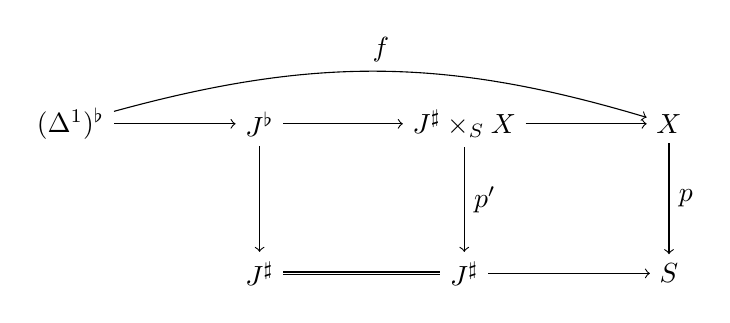
\begin{tikzpicture}
  \node (d1b) at (0,0) {$(\Delta^1)^\flat$};
  \node (jb) at (2.4,0) {$J^\flat$};
  \node (po) at (5,0) {$J^\sharp \times_S X$};
  \node (x) at (7.6,0) {$X$};
  \node (js1) at (2.4,-1.9) {$J^\sharp$};
  \node (js2) at (5,-1.9) {$J^\sharp$};
  \node (s) at (7.6,-1.9) {$S$};
  \draw[->] (d1b) -- (jb);
  \draw[->] (jb) -- (po);
  \draw[->] (po) -- (x);
  \draw[->] (jb) -- (js1);
  \draw[->] (po) -- node[right] {$p'$} (js2);
  \draw[->] (x) -- node[right] {$p$} (s);
  \draw[double] (js1) -- (js2);
  \draw[->] (js2) -- (s);
  \draw[->, bend left=16] (d1b) to node[above] {$f$} (x);
\end{tikzpicture}
\end{center}
那么 $f$ 是 $X$ 中一条带标记的边；或者，由陈述的性质 (2)，$f$ 是 $p$-余笛卡尔的。%
\footnote{译注：原书图中此对象印作 $J^{\sharp} \amalg_S X$，脱「$\times$」号；按本段正文径改。——译者注}
由于陈述的性质 (3) 提供 $p(f)$ 的一个 $p$-余笛卡尔提升 $g\colon x \to y'$，故由
\cref{lem:locally-cocartesian}，只需证明 $f$ 是\trLocallyCocartesian。由构造，$f$ 是
∞-\trCategory{} $J^\sharp \times_S X$ 中的一个\trEquivalence{}，从而是
$p'$-余笛卡尔的。特别地，它是\trLocallyCocartesian，见\cref{ex:p-prime-cocartesian-locally-cocartesian}。
\end{proof}

\begin{corollary}\label{cor:marked-cocartesian-rlp}
带标记\trSimplicialSet{}之间的一个映射 $p\colon (X, S) \to Y^\sharp$ 相对于%
\trMarkedLeftAnodyne{}映射具有\trRightLiftingProperty{}，当且仅当 $S$ 恰为所有
$p$-余笛卡尔的边，且 $p$ 是一个\trCocartesianFibration{}。
\end{corollary}

下述推论稍后会对我们有用。

\begin{corollary}\label{cor:lambda-marked-anodyne}
映射 $(\Lambda^2_0)^\sharp \amalg_{(\Lambda^2_0)^\flat} (\Delta^2)^\flat \to (\Delta^2)^\sharp$ 是\trMarkedAnodyne{}的。
\end{corollary}

\begin{proof}
我们观察到，左边是\trSimplicialSet{} $\Delta^2$，其中边 $\Delta^{\{0,1\}}$ 与
$\Delta^{\{0,2\}}$ 带标记。我们需要证明：该映射相对于满足%
\cref{prop:marked-rlp-characterization}的性质 (1)--(3) 的映射
$p\colon X \to Y$ 满足 LLP。由于该论证与\cref{prop:marked-rlp-characterization}的
证明中出现的论证类似，只是此处以 $\Lambda^2_0$ 替代了 $\Lambda^2_1$，我们把细节留作
练习。
\end{proof}

\begin{lemma}\label{lem:pushout-product-marked-left-anodyne}
一个\trMarkedLeftAnodyne{}映射与任何\trMonomorphism{}的\trPushoutProduct{}仍是\trMarkedLeftAnodyne。
\end{lemma}

\begin{proof}
关于这一结果的完整证明，我们参考 \cite[Prop.~3.1.2.3.]{Lur09}。它在精神上与我们
在证明一个\trLeftAnodyne{}/\trRightAnodyne{}/\trInnerAnodyne{}映射与一个%
\trMonomorphism{}的\trPushoutProduct{}仍是\trLeftAnodyne{}/\trRightAnodyne{}/%
\trInnerAnodyne{}时所给出的论证非常相似：首先要观察到的是：
\begin{enumerate}[label=(\alph*)]
  \item 使结论成立的诸\trMonomorphism{}所成之集是\trSaturated{}。
  \item 使结论成立的诸\trMarkedAnodyne{}映射所成之集是\trSaturated{}。
  \item \trMarkedSimplicialSet{}中的\trMonomorphism{}由映射 $(\partial\Delta^n)^\flat \to (\Delta^n)^\flat$ 与映射 $(\Delta^1)^\flat \to (\Delta^1)^\sharp$ 生成。
\end{enumerate}
我们只证明 (c)，并把其余两项留作练习。至于 (c)，显然如上所述的诸\trBoundaryInclusion{}%
生成形如 $K^\flat \to L^\flat$ 的\trMonomorphism{}。对每个带标记%
\trSimplicialSet{} $(K, M)$ 与\trSimplicialSet{}之间的每个\trMonomorphism{}%
$K \to L$，下面是一个带标记\trSimplicialSet{}的\trPushout{}：
\begin{center}
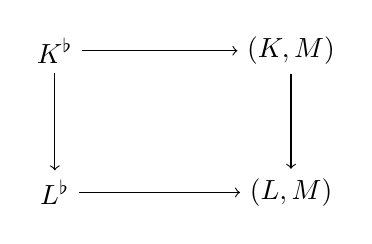
\begin{tikzpicture}
  \node (kb) at (0,0) {$K^\flat$};
  \node (km) at (3,0) {$(K, M)$};
  \node (lb) at (0,-1.8) {$L^\flat$};
  \node (lm) at (3,-1.8) {$(L, M)$};
  \draw[->] (kb) -- (km);
  \draw[->] (kb) -- (lb);
  \draw[->] (km) -- (lm);
  \draw[->] (lb) -- (lm);
\end{tikzpicture}
\end{center}
因此，右边的竖直映射由诸\trBoundaryInclusion{}生成。为了证明带标记%
\trSimplicialSet{}之间的一般\trMonomorphism{}由陈述 (c) 中出现的诸映射生成，
只需看出：对 $M \subseteq M'$，$(L, M) \to (L, M')$ 由这些映射生成。为此，
我们观察到存在一个\trPushout{}%
\begin{center}
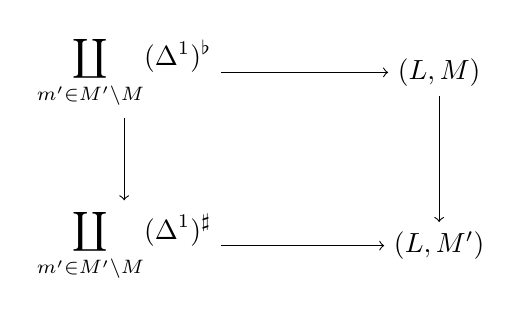
\begin{tikzpicture}
  \node (cop) at (0,0)
    {$\displaystyle\coprod_{m' \in M' \setminus M} (\Delta^1)^\flat$};
  \node (lm) at (4,0) {$(L, M)$};
  \node (cop2) at (0,-2.2)
    {$\displaystyle\coprod_{m' \in M' \setminus M} (\Delta^1)^\sharp$};
  \node (lmp) at (4,-2.2) {$(L, M')$};
  \draw[->] (cop) -- (lm);
  \draw[->] (cop) -- (cop2);
  \draw[->] (lm) -- (lmp);
  \draw[->] (cop2) -- (lmp);
\end{tikzpicture}
\end{center}
于是断言得证。

因此，只需证明：\cref{def:marked-left-anodyne}中形如 (1)--(4) 的映射与 (c) 中
出现的那种映射的\trPushoutProduct{}是\trMarkedAnodyne{}的。有八种情形需要考虑：
\begin{enumerate}[label=(\arabic*)]
  \item 我们考虑 $(\Lambda^n_i)^\flat \subseteq (\Delta^n)^\flat$ 与
        $(\partial\Delta^n)^\flat \subseteq (\Delta^n)^\flat$ 的%
        \trPushoutProduct{}。由于 $(-)^\flat$ 保持\trColimit{}，这个%
        \trPushoutProduct{}映射由对底下的诸\trSimplicialSet{}映射的%
        \trPushoutProduct{}应用 $(-)^\flat$ 给出。这又是内零调的，从而在应用
        $(-)^\flat$ 之后便成为\trMarkedAnodyne{}的。
  \item $(\Lambda^n_i)^\flat \subseteq (\Delta^n)^\flat$ 与
        $(\Delta^1)^\flat \to (\Delta^1)^\sharp$ 的\trPushoutProduct{}是一个同构，
        从而是\trMarkedAnodyne{}的。为此，注意 $n \ge 2$，故映射
        $\Lambda^n_i \to \Delta^n$ 在顶点上是同构。
  \item $K^\flat \to K^\sharp$ 与 $(\partial\Delta^n)^\flat \to (\Delta^n)^\flat$
        的\trPushoutProduct{}在 $n > 0$ 时是同构，而在 $n = 0$ 时等于映射
        $K^\flat \to K^\sharp$；无论哪种情形，它都是\trMarkedAnodyne{}的。
  \item $K^\flat \to K^\sharp$ 与 $(\Delta^1)^\flat \to (\Delta^1)^\sharp$ 的%
        \trPushoutProduct{}是映射 $(K \times \Delta^1, M) \to (K \times \Delta^1)^\sharp$，其中 $M$ 由那些 $a$ 或 $b$ 退化的对
        $(a, b)$ 给出。由于 $(K \times \Delta^1)$ 中的每个 $1$-\trSimplex{}%
        $(a, b)$ 都是 $(a, \mathrm{id})$ 与 $(\mathrm{id}, b)$ 的一个合成，且
        由于恒等是退化的，我们所感兴趣的映射是\trMarkedAnodyne{}的（添加\trMarkedEdge{}的一个
        合成是\trMarkedAnodyne{}的）。
  \item $(\Lambda^2_1)^\sharp \amalg_{(\Lambda^2_1)^\flat} (\Delta^2)^\flat \to (\Delta^2)^\sharp$ 与 $(\partial\Delta^n)^\flat \to (\Delta^n)^\flat$ 的%
        \trPushoutProduct{}在 $n \ge 1$ 时是同构，而在 $n = 0$ 时就是所给的映射，
        从而它在任何情形下都是\trMarkedAnodyne{}的。
  \item $(\Lambda^2_1)^\sharp \amalg_{(\Lambda^2_1)^\flat} (\Delta^2)^\flat \to (\Delta^2)^\sharp$ 与 $(\Delta^1)^\flat \to (\Delta^1)^\sharp$ 的%
        \trPushoutProduct{}几乎是一个同构：定义域中唯一不带标记的边（在陪域中，
        所有边都带标记）是边 $(0 \to 2,\ 0 \to 1)$。然而，这是\trMarkedEdge{}的一个
        合成，故所需的映射又是\trMarkedAnodyne{}的。
\end{enumerate}
其余的情形用\trMarkedLeftAnodyne{}映射的另一个生成集来处理最为简便，也就是说，用集合
(3$'$) 替代 (3) 来工作。关键在于，由映射
\[
(\Delta^1)^\sharp \times (\partial\Delta^n)^\flat
\cup \{0\} \times (\Delta^n)^\flat
\longrightarrow
(\Delta^1)^\sharp \times (\Delta^n)^\flat
\]
生成的\trSaturatedSet{}，与对\trMonomorphism{} $A \to B$ 由映射
\[
(\Delta^1)^\sharp \times A^\flat
\cup (\Delta^1)^\flat \times B^\flat
\longrightarrow
(\Delta^1)^\sharp \times B^\flat
\]
生成的\trSaturatedSet{}相同。
\begin{enumerate}[label=(\arabic*), resume]
  \item $(\Delta^1)^\sharp \times (\partial\Delta^n)^\flat \cup \{0\} \times (\Delta^n)^\flat \to (\Delta^1)^\sharp \times (\Delta^n)^\flat$ 与 $(\partial\Delta^n)^\flat \to (\Delta^n)^\flat$ 的\trPushoutProduct{}属于
        后一种类型。这由\trPushoutProduct{}的结合性得出：它由 $\{0\} \to (\Delta^1)^\sharp$ 与 $(\partial\Delta^n)^\flat \to (\Delta^n)^\flat$ 同其
        自身的\trPushoutProduct{}二者的\trPushoutProduct{}给出，而后者显然对某个%
        \trMonomorphism{} $A \to B$ 呈 $A^\flat \to B^\flat$ 之形。
  \item $(\Delta^1)^\sharp \times (\partial\Delta^n)^\flat \cup \{0\} \times (\Delta^n)^\flat \to (\Delta^1)^\sharp \times (\Delta^n)^\flat$ 与 $(\Delta^1)^\flat \to (\Delta^1)^\sharp$ 的\trPushoutProduct{}如前，在
        $n > 0$ 时是同构。对 $n = 0$，第一个\trPushoutProduct{}就是
        $\{0\} \to (\Delta^1)^\sharp$，于是我们得到映射
        $(\Delta^1 \times \Delta^1, M) \to (\Delta^1 \times \Delta^1)^\sharp$，
        其中 $M$ 由诸退化边以及边 $\{0\} \times \Delta^1$ 与
        $\Delta^1 \times \{\varepsilon\}$（$\varepsilon = 0$ 或 $1$）组成。
\end{enumerate}
利用性质 (3) 与\cref{cor:lambda-marked-anodyne}，我们发现这是一个%
\trMarkedLeftAnodyne{}映射的合成。
\end{proof}

由这一结果，我们可以推出下述命题。

\begin{proposition}\label{prop:functor-cocartesian-fibration}
设 $p\colon \E \to \mathcal{C}$ 是一个\trCocartesianFibration{}，并设 $K$ 是一个%
\trSimplicialSet{}。那么 $p_*\colon \E^K \to \mathcal{C}^K$ 仍是一个%
\trCocartesianFibration{}，并且一条边是 $p_*$-余笛卡尔的，当且仅当它沿 $K$ 的
任何\trObject{}的限制在 $\E$ 中的像是 $p$-余笛卡尔的。
\end{proposition}

\begin{proof}
作为\cref{lem:pushout-product-marked-left-anodyne}的一个特例，我们发现对任何%
\trMarkedLeftAnodyne{}映射 $A \to B$，映射 $A \times K^\flat \to B \times K^\flat$ 也是%
\trMarkedLeftAnodyne。利用\cref{prop:marked-rlp-characterization}，可以求解任何%
\trLiftingProblem{}%
\begin{center}
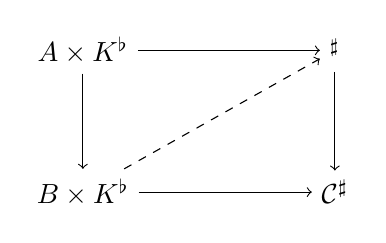
\begin{tikzpicture}
  \node (ak) at (0,0) {$A \times K^\flat$};
  \node (ef) at (3.2,0) {$\E^\sharp$};
  \node (bk) at (0,-1.8) {$B \times K^\flat$};
  \node (cf) at (3.2,-1.8) {$\mathcal{C}^\sharp$};
  \draw[->] (ak) -- (ef);
  \draw[->] (ak) -- (bk);
  \draw[->] (bk) -- (cf);
  \draw[->] (ef) -- (cf);
  \draw[->, dashed] (bk) -- (ef);
\end{tikzpicture}
\end{center}
由于 $(-)^\flat$ 是\trForgetfulFunctor{}的\trLeftAdjoint{}，这意味着
$(\E^K, S) \to (\mathcal{C}^K)^\sharp$ 相对于\trMarkedAnodyne{}映射具有%
\trRightLiftingProperty{}，其中 $S$ 由那些沿 $K$ 的任何\trObject{}的限制成为
$p$-余笛卡尔的边组成。由\cref{cor:marked-cocartesian-rlp}，$S$ 恰由诸
$p_*$-余笛卡尔边组成，且 $p_*$ 是一个\trCocartesianFibration{}。
\end{proof}

\begin{definition}\label{def:fun-mcc}
设 $p\colon \E \to \mathcal{C}$ 是一个\trCocartesianFibration{}，并设 $K$ 是一个%
\trMarkedSimplicialSet{}。我们用 $\mathrm{Fun}^{\mathrm{mcc}}(K, \E)$ 表示
$\mathrm{Fun}(K, \E)$ 中由把 $K$ 的所有\trMorphism{}送到 $\E$ 中
$p$-余笛卡尔\trMorphism{}的诸\trFunctor{}组成的满子范畴。如果 $K$ 装备了一个
映射 $f\colon K \to \mathcal{C}^\sharp$，那么我们用
$\mathrm{Fun}^{\mathrm{mcc}}_f(K, \E)$ 表示\trPullback{}%
\begin{center}
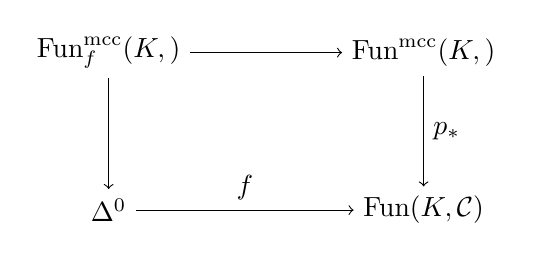
\begin{tikzpicture}
  \node (fuf) at (0,0)
    {$\mathrm{Fun}^{\mathrm{mcc}}_f(K, \E)$};
  \node (fum) at (4,0)
    {$\mathrm{Fun}^{\mathrm{mcc}}(K, \E)$};
  \node (d0) at (0,-2) {$\Delta^0$};
  \node (fkc) at (4,-2) {$\mathrm{Fun}(K, \mathcal{C})$};
  \draw[->] (fuf) -- (fum);
  \draw[->] (fuf) -- (d0);
  \draw[->] (fum) -- node[right] {$p_*$} (fkc);
  \draw[->] (d0) -- node[above] {$f$} (fkc);
\end{tikzpicture}
\end{center}
如果 $K$ 是一个通常的\trSimplicialSet{}，那么我们写 $\mathrm{Fun}^{\mathrm{cc}}(K, \E)$，
相应地写 $\mathrm{Fun}^{\mathrm{cc}}_f(K, \E)$，以指代
$\mathrm{Fun}^{\mathrm{mcc}}(K^\sharp, \E)$，相应地指代
$\mathrm{Fun}^{\mathrm{mcc}}_f(K^\sharp, \E)$。
\end{definition}

\begin{remark}\label{rem:map-notation}
在 \cite{Lur09} 中，我们所记的 $\mathrm{Fun}^{\mathrm{mcc}}(K, \E)$ 被写作
$\mathrm{Map}^\flat(K, \E^\natural)$。同样地，我们所记的
$\mathrm{Fun}^{\mathrm{mcc}}_f(K, \E)$ 被记为
$\mathrm{Map}^\flat_K(K, \E^\natural)$。
采用这一记号的缘由是，带标记\trSimplicialSet{}的\trCategory{}是\emph{\trCartesianClosed}
（cartesian closed），也就是说，对每个带标记\trSimplicialSet{} $K$，函子
$K \times -$ 容有一个\trRightAdjoint{}，记为 $X \mapsto X^K$。我们定义一个%
\trSimplicialSet{} $\mathrm{Map}^\flat(K, X)$，其 $n$-\trSimplex{} 由
$\mathrm{Hom}_{\mathrm{sSet}_+}((\Delta^n)^\flat \times K, X)$ 给出。同样地，
我们定义一个\trSimplicialSet{} $\mathrm{Map}^\sharp(K, X)$，其 $n$-\trSimplex{}%
由 $\mathrm{Hom}_{\mathrm{sSet}_+}((\Delta^n)^\sharp \times K, X)$ 给出。按照我们
先前的记号，我们有 $u(X^K) = \mathrm{Map}^\flat(K, X)$ 与
$m(X^K) = \mathrm{Map}^\sharp(K, X)$%
\footnote{译注：$u$ 与 $m$ 即本节开头的例子中那两个\trFunctor{} $\mathrm{sSet}_+ \to \mathrm{sSet}$——前者遗忘标记，后者取最小的标记。——译者注}。
\end{remark}

\begin{proposition}\label{prop:fun-mcc-trivial-fibration}
设 $p\colon \E \to \mathcal{C}$ 是一个\trCocartesianFibration{}，设
$i\colon K \to L$ 是一个\trMarkedAnodyne{}映射，并设 $f\colon L \to \mathcal{C}^\sharp$
是一个\trMorphism{}。那么，所诱导的映射
\[
\mathrm{Fun}^{\mathrm{mcc}}_f(L, \E)
\longrightarrow
\mathrm{Fun}^{\mathrm{mcc}}_{fi}(K, \E)
\]
是一个\trTrivialFibration{}。
\end{proposition}

\begin{proof}
我们需要证明，任何\trLiftingProblem{}%
\begin{center}
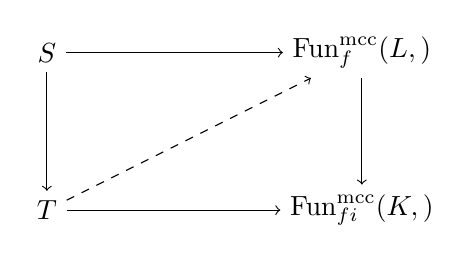
\begin{tikzpicture}
  \node (s) at (0,0) {$S$};
  \node (fl) at (4,0) {$\mathrm{Fun}^{\mathrm{mcc}}_f(L, \E)$};
  \node (t) at (0,-2) {$T$};
  \node (fk) at (4,-2) {$\mathrm{Fun}^{\mathrm{mcc}}_{fi}(K, \E)$};
  \draw[->] (s) -- (fl);
  \draw[->] (s) -- (t);
  \draw[->] (t) -- (fk);
  \draw[->] (fl) -- (fk);
  \draw[->, dashed] (t) -- (fl);
\end{tikzpicture}
\end{center}
只要 $S \to T$ 是\trSimplicialSet{}之间的一个\trMonomorphism{}，就可解。由定义
出发，这等价于\trLiftingProblem{}%
\begin{center}
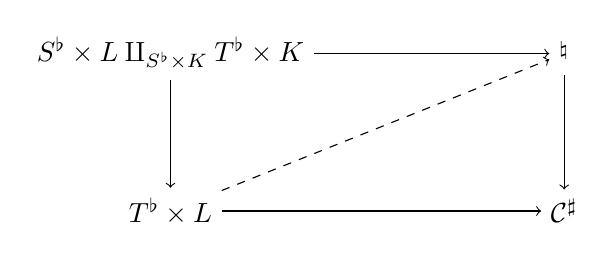
\begin{tikzpicture}
  \node (sp) at (0,0)
    {$S^\flat \times L \amalg_{S^\flat \times K} T^\flat \times K$};
  \node (ef) at (5,0) {$\E^\natural$};
  \node (tp) at (0,-2) {$T^\flat \times L$};
  \node (cf) at (5,-2) {$\mathcal{C}^\sharp$};
  \draw[->] (sp) -- (ef);
  \draw[->] (sp) -- (tp);
  \draw[->] (tp) -- (cf);
  \draw[->] (ef) -- (cf);
  \draw[->, dashed] (tp) -- (ef);
\end{tikzpicture}
\end{center}
可解。由\cref{lem:pushout-product-marked-left-anodyne}，左边的竖直映射是%
\trMarkedAnodyne{}的，故断言得证。
\end{proof}

我们从\trNguyen{}的博士论文中学到了下述引理，它在后续的内容中对我们将是
重要的，见 \cite[Lemma 3.2.3]{Ngu18}。

\begin{lemma}\label{lem:left-anodyne-sharp}
设 $K \to L$ 是一个\trLeftAnodyne{}映射。那么带标记\trSimplicialSet{}的映射
$K^\sharp \to L^\sharp$ 是\trMarkedAnodyne{}的。
\end{lemma}

\begin{proof}
首先我们断言：使 $K^\sharp \to L^\sharp$ 为\trMarkedAnodyne{}的诸\trSimplicialSet{}的%
\trMonomorphism{} $K \to L$ 所成之集是\trSaturated{}。因此，只需证明对
$0 \le i < n$，映射 $(\Lambda^n_i)^\sharp \to (\Delta^n)^\sharp$
是\trMarkedAnodyne{}的。\footnote{译注：原书此处印作 $(\Lambda^n_0)^\sharp$，与本句
量词「对 $0 \le i < n$」不配；按上下文此处理应涵盖任意内角 $\Lambda^n_i$（$\Lambda^n_0$
的情形随后另行处理），兹改 $\Lambda^n_i$。——译者注}
我们观察到，一旦 $n$ 至少为 $3$，就有 $\mathrm{sk}_1(\Lambda^n_i) = \mathrm{sk}_1(\Delta^n)$。于是，对 $n \ge 3$ 与 $0 < i < n$，我们有一个\trPushout{}%
\begin{center}
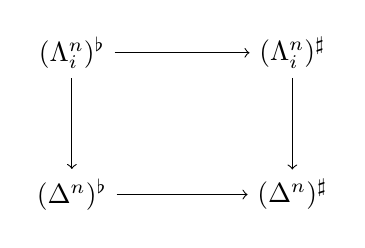
\begin{tikzpicture}
  \node (lb) at (0,0) {$(\Lambda^n_i)^\flat$};
  \node (ls) at (2.8,0) {$(\Lambda^n_i)^\sharp$};
  \node (db) at (0,-1.8) {$(\Delta^n)^\flat$};
  \node (ds) at (2.8,-1.8) {$(\Delta^n)^\sharp$};
  \draw[->] (lb) -- (ls);
  \draw[->] (lb) -- (db);
  \draw[->] (ls) -- (ds);
  \draw[->] (db) -- (ds);
\end{tikzpicture}
\end{center}
这表明右边的竖直映射是\trMarkedAnodyne{}的。类似地，存在一个\trPushout{}%
\begin{center}
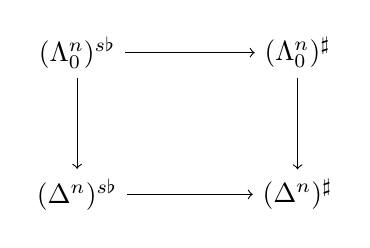
\begin{tikzpicture}
  \node (lb) at (0,0) {$(\Lambda^n_0)^{s\flat}$};
  \node (ls) at (2.8,0) {$(\Lambda^n_0)^\sharp$};
  \node (db) at (0,-1.8) {$(\Delta^n)^{s\flat}$};
  \node (ds) at (2.8,-1.8) {$(\Delta^n)^\sharp$};
  \draw[->] (lb) -- (ls);
  \draw[->] (lb) -- (db);
  \draw[->] (ls) -- (ds);
  \draw[->] (db) -- (ds);
\end{tikzpicture}
\end{center}
于是右边的竖直映射又是\trMarkedAnodyne{}的。剩下要处理的是 $n < 3$ 的情形。$n = 1$ 的
情形是清楚的，故只剩下 $n = 2$ 的情形需要处理，对此我们需要讨论 $i = 0$ 与
$i = 1$ 两种情形。存在\trPushout{}%
\begin{center}
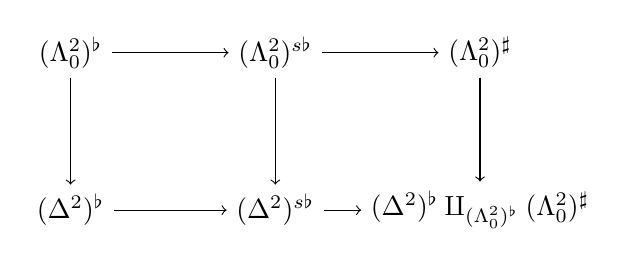
\begin{tikzpicture}
  \node (lb) at (0,0) {$(\Lambda^2_0)^\flat$};
  \node (lsb) at (2.6,0) {$(\Lambda^2_0)^{s\flat}$};
  \node (ls) at (5.2,0) {$(\Lambda^2_0)^\sharp$};
  \node (db) at (0,-2) {$(\Delta^2)^\flat$};
  \node (dsb) at (2.6,-2) {$(\Delta^2)^{s\flat}$};
  \node (po) at (5.2,-2)
    {$(\Delta^2)^\flat \amalg_{(\Lambda^2_0)^\flat} (\Lambda^2_0)^\sharp$};
  \draw[->] (lb) -- (lsb);
  \draw[->] (lsb) -- (ls);
  \draw[->] (lb) -- (db);
  \draw[->] (lsb) -- (dsb);
  \draw[->] (ls) -- (po);
  \draw[->] (db) -- (dsb);
  \draw[->] (dsb) -- (po);
\end{tikzpicture}
\end{center}
于是最右边的竖直映射是\trMarkedAnodyne{}的。由\cref{cor:lambda-marked-anodyne}，进一步的
映射
\[
(\Delta^2)^\flat \amalg_{(\Lambda^2_0)^\flat} (\Lambda^2_0)^\sharp
\longrightarrow
(\Delta^2)^\sharp
\]
也是\trMarkedAnodyne{}的，从而映射 $(\Lambda^2_0)^\sharp \to (\Delta^2)^\sharp$ 也是%
\trMarkedAnodyne{}的。对于余下的情形，我们有\trPushout{}%
\begin{center}
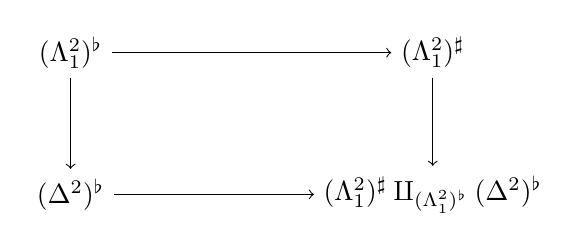
\begin{tikzpicture}
  \node (lb) at (0,0) {$(\Lambda^2_1)^\flat$};
  \node (ls) at (4.6,0) {$(\Lambda^2_1)^\sharp$};
  \node (db) at (0,-1.8) {$(\Delta^2)^\flat$};
  \node (po) at (4.6,-1.8)
    {$(\Lambda^2_1)^\sharp \amalg_{(\Lambda^2_1)^\flat} (\Delta^2)^\flat$};
  \draw[->] (lb) -- (ls);
  \draw[->] (lb) -- (db);
  \draw[->] (ls) -- (po);
  \draw[->] (db) -- (po);
\end{tikzpicture}
\end{center}
于是右边的竖直映射是\trMarkedAnodyne{}的。由定义，映射
\[
(\Lambda^2_1)^\sharp \amalg_{(\Lambda^2_1)^\flat} (\Delta^2)^\flat
\longrightarrow
(\Delta^2)^\sharp
\]
也是\trMarkedAnodyne{}的，故引理得证。
\end{proof}

有了这个引理在手，我们就有下述直接的推论，它对我们稍后而言将是非常重要的。

\begin{corollary}\label{cor:fun-cc-trivial-fibration}
设 $p\colon \E \to \mathcal{C}$ 是一个\trCocartesianFibration{}，设
$i\colon K \to L$ 是\trSimplicialSet{}之间的一个\trLeftAnodyne{}映射，并设
$f\colon L \to \mathcal{C}$ 是一个\trMorphism{}。那么，所诱导的映射
\[
\mathrm{Fun}^{\mathrm{cc}}_f(L, \E)
\longrightarrow
\mathrm{Fun}^{\mathrm{cc}}_{fi}(K, \E)
\]
是一个\trTrivialFibration{}。
\end{corollary}

\begin{proof}
这是\cref{prop:fun-mcc-trivial-fibration}在\trMarkedLeftAnodyne{}映射为 $i^\sharp\colon K^\sharp \to L^\sharp$ 时的特例，其中用到\cref{lem:left-anodyne-sharp}。
\end{proof}

如果 $f\colon \Delta^1 \to \mathcal{C}$ 是一个\trMorphism{}，那么∞-\trCategory{}%
$\mathrm{Fun}^{\mathrm{cc}}_f(\Delta^1, \E)$ 参数化 $\mathcal{C}$ 中一个给定的%
\trMorphism{}的全部 $p$-余笛卡尔提升。我们于是得到下述结果。

\begin{corollary}\label{cor:cocartesian-lifts-contractible}
设 $p\colon \E \to \mathcal{C}$ 是一个\trCocartesianFibration{}，并设
$f\colon \Delta^1 \to \mathcal{C}$ 是 $\mathcal{C}$ 中从 $x$ 到 $y$ 的一个%
\trMorphism{}。那么，通过在 $\{0\}$ 处取值给出的映射
$\mathrm{Fun}^{\mathrm{cc}}_f(\Delta^1, \E) \to \E_x$ 是一个%
\trTrivialFibration{}。特别地，\trSimplicialSet{}%
\[
\mathrm{Fun}^{\mathrm{cc}}_f(\Delta^1, \E) \times_{\E_x} \{z\}
\]
对 $\E_x$ 的每个\trObject{} $z$ 都是\trContractible{}\trKanComplex{}。
\end{corollary}

\begin{proof}
我们考虑\trPullback{}图表
\begin{center}
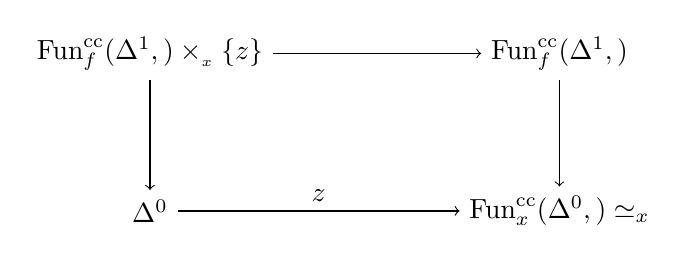
\begin{tikzpicture}
  \node (pb) at (0,0)
    {$\mathrm{Fun}^{\mathrm{cc}}_f(\Delta^1, \E) \times_{\E_x} \{z\}$};
  \node (fu) at (5.2,0)
    {$\mathrm{Fun}^{\mathrm{cc}}_f(\Delta^1, \E)$};
  \node (d0) at (0,-2) {$\Delta^0$};
  \node (fx) at (5.2,-2)
    {$\mathrm{Fun}^{\mathrm{cc}}_x(\Delta^0, \E) \simeq \E_x$};
  \draw[->] (pb) -- (fu);
  \draw[->] (pb) -- (d0);
  \draw[->] (d0) -- node[above] {$z$} (fx);
  \draw[->] (fu) -- (fx);
\end{tikzpicture}
\end{center}
其中右边的竖直映射是一个\trTrivialFibration{}，因为它是沿 $\{0\} \to \Delta^1$
限制而得到的（后者是\trLeftAnodyne{}的，所以我们可以应用\cref{cor:fun-cc-trivial-fibration}）。
因此，左边的竖直映射也是一个\trTrivialFibration{}。
\end{proof}

在本节的其余部分，我们想表明人们可以如何利用\trMarkedSimplicialSet{}来研究%
\trDwyer{}--\trKan{}\trLocalization{}。

在接下来的内容中，我们将始终把∞-\trCategories{}视为 $\Delta^0$ 之上的%
\trCocartesianFibration{}，从而 $\mathcal{C}^\natural$ 表示\trMarkedEdge{}恰为 $\mathcal{C}$
的全部\trEquivalence{}的那个带标记\trSimplicialSet{} $\mathcal{C}$。

\begin{definition}\label{def:marked-equivalence}
设 $X, Y$ 是带标记\trSimplicialSet{}。一个\trMorphism{} $f\colon X \to Y$ 称为一个
\emph{\trMarkedEquivalence{}}（marked equivalence），如果对任何∞-\trCategory{}%
$\mathcal{C}$，所诱导的映射
\[
\mathrm{Fun}^{\mathrm{mcc}}(Y, \mathcal{C})
\longrightarrow
\mathrm{Fun}^{\mathrm{mcc}}(X, \mathcal{C})
\]
是∞-\trCategories{}之间的一个\trEquivalence{}。
\end{definition}

\begin{example*}
设 $\mathcal{C}$ 是一个∞-\trCategory{}，$S$ 是一个包含全部\trEquivalence{}的%
\trMorphism{}之集，并设 $\mathcal{C}[S^{-1}]$ 是一个\trLocalization{}。那么映射
$(\mathcal{C}, S) \to \mathcal{C}[S^{-1}]^\natural$ 是一个\trMarkedEquivalence。
\end{example*}

\begin{example*}
设 $A \to B$ 是一个\trMarkedLeftAnodyne{}映射。那么 $A \to B$ 是一个\trMarkedEquivalence{}。这是%
\cref{prop:fun-mcc-trivial-fibration}的特例：我们需要证明，对每个∞-\trCategory{}%
$\E$，限制\trFunctor{}%
\[
\mathrm{Fun}^{\mathrm{mcc}}(B, \E)
\longrightarrow
\mathrm{Fun}^{\mathrm{mcc}}(A, \E)
\]
是一个\trJoyalEquivalence{}。事实上，它是一个\trTrivialFibration{}，因为对%
\trCocartesianFibration{} $\E \to \Delta^0$ 与典范映射 $*\colon B \to \Delta^0$
而言，$\mathrm{Fun}^{\mathrm{mcc}}(B, \E) = \mathrm{Fun}^{\mathrm{mcc}}_*(B, \E)$
（把 $B$ 换成 $A$ 时同理）。
\end{example*}

如同 1.3 节中那样，我们期望能够把任何映射分解成一个\trMarkedAnodyne{}映射与一个%
相对于\trMarkedAnodyne{}映射满足 RLP 的映射的合成。对形如 $X \to \Delta^0$ 的映射，我们发现
所得的映射 $\mathcal{C} \to \Delta^0$ 是一个\trInnerFibration{}，而 $\mathcal{C}$
的\trMarkedEdge{}恰好是诸\trEquivalence{}。在本书中我们将不证明下述定理。

\begin{theorem}\label{thm:marked-model-structure}
在\trMarkedSimplicialSet{}上存在一个单纯\trModelStructure{}，其\trCofibration{}是诸\trMonomorphism{}，
其\trEquivalence{}是诸\trMarkedEquivalence{}，并且其\trFibrantObject{}恰好是\trMarkedEdge{}全为%
\trEquivalence{}的∞-\trCategories{}。
\end{theorem}

\begin{corollary}\label{cor:dk-fibrant-replacement}
$\mathcal{C}$ 沿 $S$ 的一个\trDwyer{}--\trKan{}\trLocalization{}于是可以被看作
$(\mathcal{C}, S)$ 在这个\trMarkedSimplicialSet{}上的\trModelStructure{}中的一个纤维性替换。
\end{corollary}

\begin{lemma}\label{lem:marked-equiv-localization}
设 $(\mathcal{C}, S)$ 是一个带标记∞-\trCategory{}，并设 $\E$ 是一个
∞-\trCategory{}。那么存在∞-\trCategories{}之间的一个\trEquivalence{} $\mathrm{Fun}^{\mathrm{mcc}}((\mathcal{C}, S), \E) \simeq \mathrm{Fun}(\mathcal{C}[S^{-1}], \E)$。
\end{lemma}

\begin{proof}
这由\trLocalization{}的定义立即可得。
\end{proof}

更一般地，我们有下述结果。

\begin{lemma}\label{lem:marked-equiv-dk-equivalence}
设 $(\mathcal{C}, S)$ 与 $(\mathcal{D}, T)$ 是装备了映射之集的∞-\trCategories{}，
把它们视为\trMarkedSimplicialSet{}。\trMarkedSimplicialSet{}之间的一个映射
$f\colon (\mathcal{C}, S) \to (\mathcal{D}, T)$ 是一个\trMarkedEquivalence{}，当且仅当%
\trDwyer{}--\trKan{}\trLocalization{}上所诱导的映射
\[
\bar{f}\colon \mathcal{C}[S^{-1}] \xrightarrow{\ \simeq\ } \mathcal{D}[T^{-1}]
\]
是一个\trEquivalence{}。
\end{lemma}

\begin{proof}
设 $\E$ 是一个辅助∞-\trCategory{}。考虑交换图表
\begin{center}
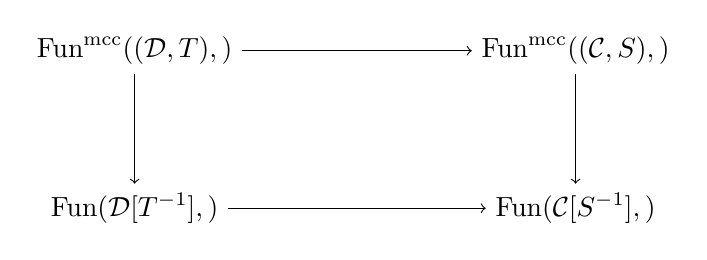
\begin{tikzpicture}
  \node (tl) at (0,0) {$\mathrm{Fun}^{\mathrm{mcc}}((\mathcal{D}, T), \E)$};
  \node (tr) at (5.6,0) {$\mathrm{Fun}^{\mathrm{mcc}}((\mathcal{C}, S), \E)$};
  \node (bl) at (0,-2) {$\mathrm{Fun}(\mathcal{D}[T^{-1}], \E)$};
  \node (br) at (5.6,-2) {$\mathrm{Fun}(\mathcal{C}[S^{-1}], \E)$};
  \draw[->] (tl) -- (tr);
  \draw[->] (tl) -- (bl);
  \draw[->] (tr) -- (br);
  \draw[->] (bl) -- (br);
\end{tikzpicture}
\end{center}
其中竖直的映射由\cref{lem:marked-equiv-localization}都是\trEquivalence{}。于是，
上面的水平映射是一个\trEquivalence{}，当且仅当下面的水平映射是一个%
\trEquivalence{}。由于 $\E$ 是任意的∞-\trCategory{}，引理得证。
\end{proof}

我们以下述结果来结束本节，这些结果描述了某些 1-\trCategories{}到相关的
Kan 充实\trCategories{}的凝聚神经的\trDwyer{}--\trKan{}\trLocalization{}。
更详细地说，对于一个\trSimplicialModelCategory{} $M$，我们令 $M^c$ 表示%
\trCofibrant{}对象（视为一个\trOrdinaryCategory{}）的\trCategory{}，并令 $M^\circ$
表示\trCofibrant{}--\trFibrantObject{}（视为一个由 $M$ 上的单纯\trModelStructure{}诱导的
Kan 充实\trCategory{}）的\trCategory{}。在 \cite{Lur17} 中，\trLurie{}构造了一个\trFunctor{}%
$\mathrm{N}(M^c) \to \mathrm{N}(M^\circ)$，它诱导一个\trFunctor{}%
$\mathrm{N}(M^c)[W^{-1}] \to \mathrm{N}(M^\circ)$，其中 $W$ 表示该%
\trModelStructure{}的\trWeakEquivalence{}之全体。

\begin{theorem}\label{thm:dk-simplicial-model}
设 $M$ 是一个\trSimplicialModelCategory{}。那么典范\trFunctor{}%
$\mathrm{N}(M^c)[W^{-1}] \to \mathrm{N}(M^\circ)$ 是∞-\trCategories{}之间的一个%
\trEquivalence{}。
\end{theorem}

\begin{corollary}\label{cor:sset-localizations}
存在∞-\trCategories{}之间的\trEquivalence{}%
$\mathrm{sSet}[\mathrm{we}^{-1}] \simeq \mathrm{Spc}$ 与
$\mathrm{sSet}[\mathrm{Joy}^{-1}] \simeq \mathrm{Cat}_\infty$。
\end{corollary}

\begin{proof}
单纯集上的 Kan--\trQuillen{}\trModelStructure{}是单纯的，并且每个对象都是%
\trCofibrant。诸\trCofibrant{}--\trFibrantObject{}正是诸\trKanComplex{}，而所诱导的 Kan 充实单纯\trCategory{}%
就是定义 $\mathrm{Spc}$ 的那一个，故第一个断言由\cref{thm:dk-simplicial-model}
得出。为了看出第二个断言，我们首先断言存在一个\trEquivalence{}%
\[
\mathrm{sSet}[\mathrm{Joy}^{-1}] \simeq \mathrm{sSet}_+[\mathrm{me}^{-1}].
\]
事实上，纤维性替换\trFunctor{}决定一个\trEquivalence{}%
$\mathrm{Cat}^1_\infty[\mathrm{Joy}^{-1}] \simeq \mathrm{sSet}[\mathrm{Joy}^{-1}]$，
见第 2 章中的\cref{lem:inclusions-induce-equivalences}。同样地，
$\mathrm{sSet}_+[\mathrm{me}^{-1}]$ 等价于诸\trFibrantObject{}在\trMarkedEquivalence{}处的%
\trLocalization{}。现在，$\mathrm{sSet}_+$ 的\trFibrantObject{}子范畴同构于
$\mathrm{Cat}^1_\infty$，其逆\trFunctor{}一方面是「遗忘标记」，另一方面是标记全部%
\trEquivalence{}。此外，由\cref{lem:marked-equiv-dk-equivalence}，∞-\trCategories{}%
之间的一个映射在视为带标记\trSimplicialSet{}的映射时，是一个\trMarkedEquivalence{}当且仅当
它是一个\trJoyalEquivalence{}。因此，我们还得到一个\trEquivalence{}%
$\mathrm{Cat}^1_\infty[\mathrm{Joy}^{-1}] \simeq \mathrm{sSet}_+[\mathrm{me}^{-1}]$。
现在，我们把\cref{thm:dk-simplicial-model}应用到如\cref{thm:marked-model-structure}
中\trMarkedSimplicialSet{}上的那个\trModelStructure{}。在最后一步，需要观察到，来自%
\trMarkedSimplicialSet{}上的单纯\trModelStructure{}的单纯充实（诸单纯映射对象由
$\mathrm{Map}^\sharp(X, Y)$ 给出，见\cref{rem:map-notation}）与用来在
第 2 章中的\cref{def:cat-infinity}里定义 $\mathrm{Cat}_\infty$ 的充实是同一个
充实。
\end{proof}

\begin{remark}\label{rem:dual-lur17}
除了诉诸关于\trSimplicialModelCategory{}的一般结果之外，人们也可以直接诉诸
\cite[Proposition 1.3.4.7]{Lur17} 的一个对偶版本（使用路对象而非柱对象），并以
这种方式推出\cref{cor:sset-localizations}。我们指出，\cite[Proposition
1.3.4.7]{Lur17} 进入了\cref{thm:dk-simplicial-model}的证明。
\end{remark}
